% This is the Reed College LaTeX thesis template. Most of the work
% for the document class was done by Sam Noble (SN), as well as this
% template. Later comments etc. by Ben Salzberg (BTS). Additional
% restructuring and APA support by Jess Youngberg (JY).
% Your comments and suggestions are more than welcome; please email
% them to cus@reed.edu
%
% See https://www.reed.edu/cis/help/LaTeX/index.html for help. There are a
% great bunch of help pages there, with notes on
% getting started, bibtex, etc. Go there and read it if you're not
% already familiar with LaTeX.
%
% Any line that starts with a percent symbol is a comment.
% They won't show up in the document, and are useful for notes
% to yourself and explaining commands.
% Commenting also removes a line from the document;
% very handy for troubleshooting problems. -BTS

% As far as I know, this follows the requirements laid out in
% the 2002-2003 Senior Handbook. Ask a librarian to check the
% document before binding. -SN

%%
%% Preamble
%%
% \documentclass{<something>} must begin each LaTeX document
\documentclass[12pt,twoside]{templates/facsothesis}
% Packages are extensions to the basic LaTeX functions. Whatever you
% want to typeset, there is probably a package out there for it.
% Chemistry (chemtex), screenplays, you name it.
% Check out CTAN to see: https://www.ctan.org/
%%
\ifxetex
  \usepackage{polyglossia}
  \setmainlanguage{spanish}
  % Tabla en lugar de cuadro
  \gappto\captionsspanish{\renewcommand{\tablename}{Tabla}
          \renewcommand{\listtablename}{Índice de tablas}}
\else
  \usepackage[spanish,es-tabla]{babel}
\fi
%\usepackage[spanish]{babel}
\usepackage{graphicx,latexsym}
\usepackage{amsmath}
\usepackage{amssymb,amsthm}
\usepackage{longtable,booktabs,setspace}
\usepackage{chemarr} %% Useful for one reaction arrow, useless if you're not a chem major
\usepackage[hyphens]{url}
% Added by CII
%\usepackage{hyperref}
\usepackage[colorlinks = true,
            linkcolor = blue,
            urlcolor  = blue,
            citecolor = blue,
            anchorcolor = blue]{hyperref}
\usepackage{lmodern}
\usepackage{float}
\floatplacement{figure}{H}
% End of CII addition
\usepackage{rotating}
\usepackage{placeins} % para fijar la posición de las tablas con \FloatBarrier


\usepackage[]{natbib}


% Next line commented out by CII
%\usepackage{biblatex}
%\usepackage{natbib}
% Comment out the natbib line above and uncomment the following two lines to use the new
% biblatex-chicago style, for Chicago A. Also make some changes at the end where the
% bibliography is included.
%\usepackage{biblatex-chicago}
%\bibliography{thesis}


% Added by CII (Thanks, Hadley!)
% Use ref for internal links
\renewcommand{\hyperref}[2][???]{\autoref{#1}}
\def\chapterautorefname{Chapter}
\def\sectionautorefname{Section}
\def\subsectionautorefname{Subsection}
% End of CII addition

% Added by CII
\usepackage{caption}
\captionsetup{width=5in}
% End of CII addition

% \usepackage{times} % other fonts are available like times, bookman, charter, palatino

% Syntax highlighting #22

% To pass between YAML and LaTeX the dollar signs are added by CII
\title{¿Quién justifica qué? El papel del sentido de (in)justicia en las justificaciones de violencia en contexto de protesta}
\author{Martín Venegas Márquez}
% The month and year that you submit your FINAL draft TO THE LIBRARY (May or December)
\date{2021-08-05}
\division{}
\advisor{Profesor/a guía: Juan Carlos Castillo}
\institution{Universidad de Chile}
\degree{Memoria de Título - Carrera de Sociología}
%If you have two advisors for some reason, you can use the following
% Uncommented out by CII
% End of CII addition

%%% Remember to use the correct department!
\department{}
% if you're writing a thesis in an interdisciplinary major,
% uncomment the line below and change the text as appropriate.
% check the Senior Handbook if unsure.
%\thedivisionof{The Established Interdisciplinary Committee for}
% if you want the approval page to say "Approved for the Committee",
% uncomment the next line
%\approvedforthe{Committee}

% Added by CII
%%% Copied from knitr
%% maxwidth is the original width if it's less than linewidth
%% otherwise use linewidth (to make sure the graphics do not exceed the margin)
\makeatletter
\def\maxwidth{ %
  \ifdim\Gin@nat@width>\linewidth
    \linewidth
  \else
    \Gin@nat@width
  \fi
}
\makeatother

%Added by @MyKo101, code provided by @GerbrichFerdinands

\setlength\parindent{0pt}


% Added by CII

\providecommand{\tightlist}{%
  \setlength{\itemsep}{0pt}\setlength{\parskip}{0pt}}

\Acknowledgements{

}

\Dedication{

}

\Preface{

}

\Abstract{

}

	\usepackage{booktabs}
 \usepackage{longtable}
 \usepackage{array}
 \usepackage{multirow}
 \usepackage{wrapfig}
 \usepackage{float}
 \usepackage{colortbl}
 \usepackage{pdflscape}
 \usepackage{tabu}
 \usepackage{threeparttable}
 \usepackage{threeparttablex}
 \usepackage[normalem]{ulem}
 \usepackage{makecell}
 \usepackage{xcolor}
% End of CII addition
%%
%% End Preamble
%%
%
\let\chaptername\relax
\begin{document}
\bibliographystyle{apalike}
% Everything below added by CII
  \maketitle

\frontmatter % this stuff will be roman-numbered
\pagestyle{empty} % this removes page numbers from the frontmatter



%  \hypersetup{linkcolor=black}
  \setcounter{tocdepth}{1}
  \setlength{\parskip}{0pt}
  \tableofcontents

\setlength\parskip{1em plus 0.1em minus 0.2em}

  \listoftables

  \listoffigures



\mainmatter % here the regular arabic numbering starts
\pagestyle{fancyplain} % turns page numbering back on

\hypertarget{resumen}{%
\chapter*{Resumen}\label{resumen}}
\addcontentsline{toc}{chapter}{Resumen}

La vida en democracia consiste en convivir con la violencia al plantear limites para su uso, tornándose la justificación de la violencia una discusión relevante en la agenda pública. En Chile, en los últimos años y especialmente desde el \emph{estallido social} se ha visto un incremento en las justificaciones de violencia asociadas a las tácticas de protesta (violencia por el cambio social), y una baja en la violencia asociada a la represión policial (violencia por el control social). Considerando que la justificación de la violencia amenaza con la convivencia pacífica, es que se torna relevante hacerse la pregunta por ¿qué lleva a las personas a justificar la violencia?. La literatura empírica ha generado evidencia en torno a las teorías del conflicto con enfoque criminológico, las teorías de la dominancia social y del autoritarismo de derecha y la de justicia procesal. La literatura teórica ha relevado el rol que tienen las experiencias de injusticia. En base en los hallazgos hasta ahora, se propone la aplicación del marco de la justicia distributiva para ampliar el estudio empírico entre la justicia y las justificaciones de violencia. El argumento principal del estudio es que el sentido de (in)justicia en la distribución de ingresos lleva a justificar más la violencia por el cambio y menos por el control social. También se estudiará el rol de la justicia procesal y el carácter de grupos desventajados.

\hypertarget{agradecimientos}{%
\chapter*{Agradecimientos}\label{agradecimientos}}
\addcontentsline{toc}{chapter}{Agradecimientos}

\hypertarget{introducciuxf3n}{%
\chapter{Introducción}\label{introducciuxf3n}}

La violencia es uno de los componentes principales de la experiencia humana. Se presenta de distintas formas y en distintos niveles; está en la guerra y en los conflictos raciales, así como también en el crimen y las relaciones interpersonales. Es un fenómeno que tiene implicancias en todas las esferas de la vida: causa sufrimiento, humillación y, muchas veces, va aparejada de grandes cambios sociales. Todas las sociedades democráticas deben enfrentarse al desafío de disminuir los niveles de violencia \citep{Gerber2017, Keane2004}. Es más, según algunos pensadores de la modernidad como Thomas Hobbes o Max Weber, la centralización y racionalización de la violencia es constitutiva a la formación de los Estados modernos. Otros pensadores más contemporáneos han sido más enfáticos en la idea de que la violencia se ha ido democratizando con el paso del tiempo \citep{Keane2004}, lo cual tiene una gran implicancia: la coexistencia entre violencia y democracia, o dicho de otra manera, la vida en democracia consiste en plantear limites sobre qué tipo de violencias son justificables y cuáles no. Generalmente, la violencia se concibe como el daño físico ejercido de manera intencional, y la justificación de la violencia como la argumentación de que esa acción violenta trae alguna consecuencia que compensa el acto mismo \citep{Frazer2020}. La concepción del Estado como el monopolio de la violencia \citep[1919{]}]{Weber1996} establece que son los agentes representantes del Estado quienes tienen el derecho legítimo al uso de la violencia; cómo su tarea es mantener el orden social, el uso de la violencia les es justificado. Sin embargo, tanto la literatura como los procesos sociopolíticos recientes han demostrado que este no es siempre el caso. Existen una serie de otras situaciones en las que la violencia podría ser justificada por parte de la población.

El que la gente justifique la violencia en los tiempos de las democracias contemporáneas parece algo paradójico, más aun considerando los esfuerzos a nivel internacional que se han hecho para erradicar la violencia \citep{WHO2014, WHO2010, WHO2009}. No obstante, procesos sociopolíticos recientes como las movilizaciones masivas del 2019 en Chile hacen pensar que esta no es una idea tan lejana a la realidad. El llamado \emph{estallido social} fue un proceso caracterizado por violaciones sistemáticas a los derechos humanos por parte de la policía \citep{Human2019, ONU2019, Defensoria2020, Amnistia2020}, así como también por un alza en la cantidad de protesta violenta (en comparación a otro tipo de conflictos en los últimos 10 años en el país) \citep{Joignant2020}. Este evento permite plantear dos reflexiones. Por un lado, pareciese ser que la violencia ejercida por agentes estatales no siempre está justificada. Por otro lado, que una gran cantidad de manifestantes consideró a la violencia como una vía aceptable de manifestación. De hecho, las encuestas muestran que la violencia como forma de protesta tuvo un incremento en sus niveles de justificación, mientras que la aprobación a la violencia policial disminuyó considerablemente \citep{ELSOC2019}. Si un 18.7\% de las personas encuestadas el 2016 señalaba que, si se justificaba el que estudiantes lancen piedras a carabineros en forma de protesta, el 2019 un 26.8\% lo justificaba, por otro lado, mientras el 2016 un 34.9\% de los encuestados señalaba que se justif
ica que carabineros usen la fuerza para reprimir una marcha pacífica, este porcentaje desciende a 21.2\% el 2019. El ascenso en los niveles de justificación de la violencia se torna especialmente relevante si se tiene en consideración que aquellos que la justifican son más tendientes a ejercerla \citep{Markowitz2001}, o a condonar el actuar violento de otros miembros de la sociedad \citep{Kalmoe2014}. La consecuencia de esta relación es una potencial escala de violencia que amenaza la convivencia pacífica \citep{Gerber2017}. Ante esta problemática, se abren las interrogantes sobre quiénes y por qué razones las personas justifican la violencia.

Los estudios que han buscado responder estas preguntas han partido de una dicotomía que distingue la violencia de acuerdo con sus fines \citep{Blumenthal1972}. Es decir, si la violencia tiene por finalidad mantener el control social, como, por ejemplo, el actuar de agentes policiales. O si más bien, la violencia está dirigida al cambio social, como es el caso de manifestantes. Aquí, los estudios han girado en torno a tres teorías. La literatura criminológica, especialmente en los Estados Unidos, ha generado evidencia sistemática a favor de la teoría del conflicto \citep{Thompson2004}. En base a la idea de que la policía está al servicio de los grupos con mayor estatus a fin de mantener las jerarquías, es que minorías raciales y grupos de menor estatus tienden a apoyar menos la violencia de parte de la policía. En cambio, las explicaciones más psicológicas se han basado en las teorías de la dominancia social \citep{Sidanius1999} y del autoritarismo de derecha \citep{Altemeyer1988}, hallando que estas ideologías se encuentran positivamente relacionadas al apoyo de la violencia por parte de la policía. Siguiendo en psicología, en los últimos años se han incorporado las justificaciones de la violencia al marco de la justicia procesal \citep{Tyler2006}, encontrando que aquellas personas que conciben a la policía como un actor legitimo en la medida que es justo en los procedimientos asociados a su rol, es que justifican más la violencia policial y menos la violencia como protesta.

Las perspectivas que se han empleado para estudiar la justificación de la violencia no responden a un marco de investigación unificado, sino a una acumulación de estudios que han puesto a prueba distintas teorías. Como se señaló, en los últimos ha tomado fuerza la aplicación del marco teórico de la justicia procesal de \citet{Tyler2006}. Distintos estudios han seguido esta línea de estudio, contribuyendo con hallazgos prometedores para el desarrollo de una agenda de investigación \citep[e.g.][]{Puga2016, Gerber2016, Gerber2017a, Gerber2017}. Sin perjuicio de lo anterior, este escrito parte de la base de que la justicia procesal es solo una de las formas de justicia que pueden ser importantes para explicar las dinámicas de la justificación de la violencia, tanto por el control social como por el cambio social. Es por eso que, una de las primeras intenciones de este trabajo es ampliar la relación empírica entre justicia y violencia.

La justicia y la violencia tienen una relación estrecha en la literatura. Autores como \citet{Bufacchi2007} proponen que la teorización de ambos conceptos parte del mismo punto: los sentimientos de humillación. De forma similar, la teoría de la violencia estructural de \citet{Galtung1969} propone una equivalencia entre las injusticias sistemáticas y la violencia estructural. Así también, la clásica propuesta de \citet{BarringtonMoore1978} sobre la injusticia como base social de las revueltas y los conflictos violentos es otro ejemplo de esta estrecha relación. No solo se ha propuesto la relación entre la justicia y la acción violenta, sino que también con la justificación de la violencia. La teoría política y la filosofía han postulado que las experiencias y sentimientos de injusticia son un determinante sustancial en que los afectados vean a la violencia como una alternativa de acción \citep[e.g][]{Wells1970, Bufacchi2007}. La noción básica de este postulado es que un acto de violencia se justifica si es que permite enmendar una situación de injusticia, o que con su ejercicio es posible llegar a un estado más justo que al comienzo. La pregunta que este postulado deja sobre la mesa es ¿sobre qué tipo de justicia estamos hablando? En este trabajo, me baso en la conceptualización de \citet{Sabbagh2016} sobre cuatro formas de justicia: procesal, distributiva, retributiva y restaurativa y propongo que es posible ampliar la relación empírica entre justicia y justificación de la violencia al indagar en la dimensión de la justicia distributiva.

¿Por qué la dimensión de la justicia distributiva podría ayudar a comprender la justificación de la violencia? En sociología y otras disciplinas afines existe una amplia gama de estudios sobre los efectos de la desigualdad. En particular, los estudiosos que se han centrado explicar los efectos de la desigualdad económica en los niveles de violencia política de una sociedad han hallado que, en general, sociedades con mayor desigualdad económica tienden a tener más conflictos violentos \citep{Ostby2013}. En complemento a esta idea, en el campo de estudios sobre justicia social empírica han habido grandes esfuerzos en el estudio de los efectos socio conductuales del sentido de (in)justicia, especialmente de los sentimientos de injusticia que refieren a la distribución justa de los recursos de una sociedad. Dentro de las teorías sobre la justicia distributiva, la teoría de la evaluación de justicia de \citet{Jasso1980} ha sido más enfática al incluir la pregunta por las consecuencias del sentido de (in)justicia como una de las cuatro preguntas que guían la agenda de justicia distributiva. En este marco de estudios, se destaca la fuerza socio conductual que alberga el sentido de (in)justicia, complementando las propuestas de otras disciplinas. En consecuencia, propongo que el marco de la justicia distributiva puede ser de utilidad para estudiar las justificaciones de violencia por dos razones. Primero, dada la fuerza socio conductual que tiene el sentido de (in)justicia, y la ya mencionada relación que existe entre la justificación y la acción violenta, tiene sentido proponer que la fuerza socio conductual del sentido de justicia también tiene un efecto en la justificación de la violencia. Segundo, la agenda de justicia distributiva, y específicamente la teoría de la evaluación de justicia, ofrece la posibilidad de estudiar empíricamente la relación entre el sentido de (in)justicia y las justificaciones de la violencia.

Además de los aportes que hace el marco de la justicia distributiva en si mismo, el caso de Chile se torna especialmente relevante para estudiar la relación entre el sentido de (in)justicia y las justificaciones de violencia. Chile es un país caracterizado por la desigualdad económica y social \citep{PNUD2017}. La lectura que se ha hecho del estallido social es que fue la acumulación de distintas desigualdades que la población concebía como injustas lo que llevó a las grandes movilizaciones del 2019, Inclusive, años atrás el informe de \citet{PNUD2017} diagnosticaba las diversas desigualdades socioeconómicas que vivía el país, tales como las brechas de ingreso o las diferencias de trato. De esta manera, tiene sentido plantear que, en uno de los países más desiguales de América Latina, los sentimientos de injusticia jugaron un rol importante en que la gente justificara la violencia que caracterizó el Estallido Social. La intención de este escrito no es explicar las movilizaciones del 2019, sino usarlas como caso paradigmático en donde esta relación podría ser particularmente fuerte.

En resumen, la hipótesis central de este escrito es que el sentido de (in)justicia, específicamente relacionado a los ingresos, tiene un efecto positivo en las justificaciones de violencia por el cambio social, y un efecto negativo en la justificación de la violencia por el control social. En este caso, me centraré en la violencia en el contexto de protesta, por lo que las situaciones que este estudio abarca tienen que ver con dos actores principales: carabineros y manifestantes. Además de esta hipótesis principal, basándome en la idea de que suelen ser los más desfavorecidos los que experimentan la injusticia, analizaré el potencial rol mediador del estatus en las justificaciones de violencia en contexto de protesta.

El principal aporte a la literatura que este trabajo busca lograr es la ampliación de la relación empírica entre justicia y violencia, por la vía de la inclusión de la dimensión distributiva. Aparte de esta propuesta, este estudio utilizará los datos de la Encuesta Longitudinal Social de Chile (ELSOC), por lo que permitirá ser una base empírica para el planteamiento de hipótesis de tipo longitudinal. Por lo demás, este es el primer trabajo que se propone indagar en las determinantes que llevaron a los chilenos a los niveles de justificación de violencia vistos el 2019, por lo que esta información puede ser evidencia relevante para el desarrollo de políticas públicas.

Este escrito tendrá cinco secciones. Primero, se tratará con más de detalle el concepto de violencia y su justificación. Segundo, se revisarán los predictores asociados a la justificación de la violencia según la literatura. Tercero, se revisarán los datos y el método a utilizar para la elaboración de resultados. Cuarto se presentarán los análisis. Por último, se presentan las discusiones y conclusiones de los hallazgos con relación a la literatura existente. Al final de este trabajo el lector tendrá conocimiento de algunas potenciales explicaciones de las justificaciones de violencia posterior al estallido social en Chile.

\hypertarget{preguntas-y-objetivos-de-investigaciuxf3n}{%
\chapter{Preguntas y objetivos de investigación}\label{preguntas-y-objetivos-de-investigaciuxf3n}}

La pregunta que orienta la presente investigación es la siguiente:

\begin{quote}
¿Cuál es la relación entre el sentido de (in)justicia y las justificaciones de la violencia en contexto de protesta, tanto por el cambio social, como por el control social, en Chile al año 2019?
\end{quote}

El objetivo general subsecuente es:

\begin{quote}
\textbf{Determinar} la relación entre el sentido de (in)justicia y las justificaciones de la violencia en contexto de protesta, tanto por el cambio social, como por el control social, en Chile al año 2019
\end{quote}

Los objetivos específicos que permitirán dar una respuesta a la pregunta de investigación son los siguientes:

\begin{itemize}
\item
  \textbf{Explicar} la relación entre la brecha de ingresos justa y las justificaciones de violencia en contexto de protesta, tanto por el cambio social, como por el control social.
\item
  \textbf{Explicar} la relación entre las percepciones del trato justo y las justificaciones de violencia en contexto de protesta, tanto por el cambio social, como por el control social.
\item
  \textbf{Explorar} el rol mediador del estatus en la relación entre el sentido de (in)justicia y las justificaciones de violencia en contexto de protesta, tanto por el cambio, como por el control social.
\end{itemize}

Las hipótesis girarán en torno a los tres objetivos específicos, y se listarán de al final de la sección de antecedentes.

\hypertarget{antecedentes-conceptuales-y-empuxedricos}{%
\chapter{Antecedentes conceptuales y empíricos}\label{antecedentes-conceptuales-y-empuxedricos}}

Previo a entrar a fondo en la revisión de los conceptos principales de este estudio (sentido de (in)justicia y justificaciones de violencia), se torna relevante especificar una definición de la violencia. A modo de adelanto, este estudio entiende la violencia como el ejercicio del daño físico que se causa de forma intencional. En el caso de la protesta, implica acciones como el lanzamiento de piedras de manifestantes o la represión por parte de carabineros. Sin embargo, existen muchas definiciones del concepto de violencia, por lo que comenzaré resumiendo las principales aproximaciones.

Una vez entendido el concepto de violencia pasaré a revisar qué significa que las personas justifiquen la violencia. A su vez repasaré las principales teorías que han indagado en los determinantes para la justificación de la violencia.

La otra sección del apartado de antecedentes consistirá en describir la idea del sentido de (in)justicia y por qué puede ser relevante para entender las dinámicas de la justificación de la violencia en contexto de protesta. Terminaré la sección de antecedentes sintetizando lo que ha sido la relación entre justicia y violencia en la literatura, y acabaré planteando las hipótesis que guían el estudio.

\hypertarget{violencia-desglosando-el-concepto}{%
\section{Violencia, desglosando el concepto}\label{violencia-desglosando-el-concepto}}

La violencia es, sin duda, uno de los conceptos más complejos en el estudio de la sociedad. Distintos académicos han trabajado a fin de responder lo que se considera una de las grandes preguntas filosóficas: ¿qué es la violencia? Estos esfuerzos han llevado a una amplia producción académica que ha buscado sintetizar esta complejidad \citep[e.g.][]{Kurt2008, Heitmeyer2005, Bufacchi2009a}. El punto de partida de toda esta empresa intelectual es siempre el mismo: la definición de violencia no es solo una, sino que viene en muchos tipos y formas. La violencia puede estar en las micro interacciones o en las grandes estructuras sociales, puede ocurrir en las relaciones de pareja, en el trabajo, en la familia y en la escuela, o en la cultura y las instituciones. Violencia puede ser desde un marido que golpea a su mujer, hasta la represión policial en el contexto de protesta; pueden ser las prácticas coloniales que marginalizan a ciertos grupos minoritarios o las estructuras de injusticia en una sociedad. En síntesis, la violencia abunda, al igual que las tipologías que existen para entenderla. Ante tal complejidad es que un estudio sobre la violencia, especialmente uno de carácter empírico, debe dejar bien establecida qué es la violencia y qué tipo de violencia se está estudiando.

Una de las distinciones base en la literatura refiere al tipo de enfoque que se adopta al momento de definir la violencia. Es decir, ¿cuál es el criterio que se prioriza al momento de definir si algo es violento o no? Los académicos han coincidido en que la gran mayoría de las definiciones que se pueden encontrar se centran o en el uso de la fuerza física o en la violación de derechos, dando pie a los dos grandes enfoques existentes \citep{Bufacchi2005}. Por un lado, está el enfoque minimalista y, por otro lado, el enfoque comprehensivo. Cada aproximación cuenta con sus ventajas y desventajas, las que se exponen a continuación.

El enfoque minimalista comprende la violencia como un acto de fuerza física intencional que causa daño en quien lo recibe. Por ejemplo, un sujeto que golpea a otro hiriéndolo intencionalmente. Este es el enfoque más recurrente, tanto en el sentido común, como en la investigación empírica y teórica. Su ventaja recae en qué, dada la estrechez de su definición, hace a la violencia un fenómeno fácilmente delimitable y abordable para la investigación empírica. Además, al incluir la idea de intencionalidad permite una discusión más clara sobre la evaluación moral del acto. Autores como \citet{Keane2004} o \citet{Coady2008} llaman a preservar este tipo de definiciones por su fácil operacionalización. Sin embargo, autores como \citet{Galtung1969} o \citet{Bufacchi2007} argumentan que delimitar la violencia hacia la fuerza física, la intencionalidad y el daño lleva a ignorar una serie de dimensiones de la violencia igualmente importantes, tales como la violencia psicológica, simbólica o estructural.

Un enfoque más estrecho relacionado a la definición minimalista es el \emph{legitimista}. El enfoque legitimista parte de la base que el criterio definitorio de la violencia es el uso de la fuerza física intencional, pero añade la condición de que debe ser ejercida por perpetradores no legítimos para ser considerada violencia. En otras palabras, restringe la definición de violencia hacia actores no estatales. De esta manera, las autoridades legítimas como policías o militares no cometen violencia, sino que hacen uso de la fuerza con tal de mantener el orden social. Esta postura ha sido defendida por autores como \citet{Hook1976}, caracterizando una visión conservadora sobre la violencia. Desde este punto de vista, dimensiones como la violencia institucional son de plano equivocadas. Por ende, desde este enfoque la violencia utilizada desde agentes privados es eminentemente peyorativa.

En contraste al enfoque minimalista, el enfoque comprehensivo pone el foco en la idea de violación. Violar significa la transgresión de un límite o norma \citep{Bufacchi2005, Bufacchi2007}, siendo la pregunta consiguiente ¿qué es violado? Autores como \citet{Gerd1969} responden definiendo la violencia como la violación de las primeras tres reglas morales: no matar, no causar daño, no deshabilitar. No obstante, la respuesta más común es que un acto de violencia es aquel que viola los derechos más básicos de un individuo, así como el derecho a la vida o a la seguridad etc. \citep{Copoeru2020}. Autores como \citet{Demirbas2019} han sido más enfáticos en entender la violencia como la violación a los derechos humanos. La ventaja de este enfoque es que logra abarcar las dimensiones que la versión minimalista de la violencia dejaba de lado: la violencia no directamente visible, inserta en la estructura social, las instituciones o la cultura, lo que \citet{Zizek2008} ha llamado violencia objetiva. Esta perspectiva prioriza la visión que tienen las víctimas de injusticias sobre la violencia, ya que son sus derechos los violados. En esa línea, es que \citet{Galtung1969} o \citet{Bourdieu1991} han trabajado en torno a conceptos como violencia estructural o violencia simbólica, respectivamente. La desventaja de esta aproximación es su carácter omniabarcante, autores como \citet{Bufacchi2005} plantean que este enfoque puede llevar a concebir la violencia como todo lo moralmente incorrecto y privándolo de su utilidad conceptual. La violencia pasa a ser un detector de injusticas más que un concepto con utilidad para la reflexión teórica y la investigación empírica \citep{Arostegui1994}.

En síntesis, los componentes principales del enfoque minimalista son la fuerza, la intencionalidad y el daño, siendo una definición que se centra en el acto directo del perpetrador. En cambio, el enfoque comprehensivo se centra en la violación de los limites o las normas, usualmente de derechos, poniendo el foco en la vivencia de la víctima. Dada su claridad conceptual, y a falta de una base empírica sobre qué es lo que entienden los chilenos por violencia, es que este trabajo se basa en una definición minimalista de la violencia. Sin embargo, aún queda por conceptualizar cuál es la situación en la que se enmarca el acto de violencia, cuestión que se especificará posterior a entender la definición base del objeto de estudio de este trabajo: la justificación de la violencia.

\hypertarget{justificaciuxf3n-de-la-violencia}{%
\section{Justificación de la violencia}\label{justificaciuxf3n-de-la-violencia}}

La justificación de la violencia parte de la base que hay algo en estos actos que los hace desvincularse de una acción meramente arbitraria \citep{Basaure2020}. Generalmente, ese algo es que las consecuencias del acto traen consigo algún bien \citep{Frazer2019}. Es decir, quienes justifican la violencia son aquellas personas que consideran que las consecuencias generadas por el acto violento traerán un bien que compense el daño efectuado durante el proceso. El conocido dicho \emph{el fin justifica los medios} representa bastante bien esta postura. Enfocar la justificación de la violencia a partir de sus consecuencias significa concebir la violencia como un acto instrumental \citep{Blumenthal1972, Arendt2005}, o sea, que cuenta con un fin que orienta su actuar. Por ende, la discusión sobre la justificación de la violencia gira en torno a cuáles son esos fines por los cuales las personas estarían dispuestas a utilizar medios violentos para conseguirlo.

El campo de estudios sobre la justificación de la violencia se puede dividir en dos grandes áreas disciplinares. Primero están los estudios en teoría política, filosofía y ética, los cuales han contribuido con reflexiones desde un punto de vista normativo. Estos trabajos giran en torno a una gran pregunta ¿puede la violencia ser justificada? Generalmente esta pregunta se sitúa en el campo de la violencia política, indagando en las condiciones, los argumentos y los principios por los cuáles se podría argumentar que la violencia revolucionaria o la violencia en contexto de protesta son moralmente defendibles \citep{Demirbas2019, Frazer2019, Gerd1969, Hills2011, Keane2004, Magil2008, Nielsen1981, Wells1970}. Las discusiones en torno al argumento \emph{ticking bomb} \citep[ver][]{APT2007, Bufacchi2006} o al asesinato de Hitler \citep[ver][]{Dean2005, Frazer2019} son algunos ejemplos de estas situaciones. Si bien no es la prioridad de este trabajo el enfoque normativo, si sienta una base importante para su estudio empírico, especialmente considerando que muchos estudios empíricos sobre violencia han caído en confusiones conceptuales por no considerar el trabajo teórico en el área \citep{Bufacchi2007}. Segundo, está el estudio empírico sobre los factores que llevan a las personas a justificarla violencia. Será en esta segunda área temática donde este trabajo se enmarca, y en donde sentará sus aportes. Dado este enmarque, es que un breve recorrido por lo que han sido las principales agendas de investigación se presenta a continuación.

El primer estudio empírico que trata las justificaciones de violencia desde un enfoque instrumental es \citet{Blumenthal1972}. Este estudio sienta las bases al conceptualizar la violencia de acuerdo a dos fines contrapuestos: por el control social y por el cambio social. A grandes rasgos, la violencia por el control social son aquellas acciones orientadas a la mantención de las jerarquías en la sociedad y la violencia por el cambio social las acciones que buscan generar un cambio en esas jerarquías. En base a esta distinción, los enfoques se han diversificado. Por un lado, la violencia por el control social puede ser ejercida por agentes privados o públicos. Cuando se trata de agentes privados, el estudio se ha centrado en actitudes hacia el castigo y la justificación de linchamientos por parte de la ciudadanía \citep[e.g.][]{Gerber2012, Gerber2016, Puga2016}. Cuando se trata de agentes públicos, se ha acuñado el concepto de violencia institucional, entendida como las medidas que toma el Estado para reprimir principios de libertad y justicia con el fin de mantener el orden social \citep{Nielsen1981}. Ejemplos de este tipo de violencia son los castigos penales o la violencia policial \citep{Puga2016}. Por otro lado, la violencia por el cambio social puede ser a nivel revolucionario, o más bien tácticas de protesta que buscan generar cambios dentro de la sociedad \citep{Nielsen1981}. La violencia revolucionaria se refiere al uso de la violencia para lograr cambios estructurales a nivel político, social y económico \citep[ver][]{Nielsen1977, Sune2010, Edyvane2020}. La violencia dentro del Estado para el cambio social apunta a la generación de cambios que no buscan la transformación total en el corto plazo. Este trabajo busca estudiar las justificaciones de violencia por el control social ejercida por agentes públicos (carabineros) y las justificaciones de violencia por el cambio social a nivel de tácticas de protesta (manifestantes).

Si bien esta es una distinción clave en los estudios contemporáneos de la justificación de la violencia, no fue retomada cómo tal hasta los años 2000 por autores cómo \citet{Jackson2013} o \citet{Gerber2016}. Es más, gran parte de los aportes provienen de la literatura criminológica en los Estados Unidos bajo el estudio de conceptos como \emph{actitudes o apoyo hacia el uso de la fuerza por parte de la policía}, y no de violencia como tal. En esta línea muchos artículos se centraron en los factores que lleva a la gente a apoyar uso de la fuerza policial \citep{Gamson1970, Arthur1993, Arthur1994, Thompson2004, Perkins2006, Johnson2009} o también en el desarrollo de escalas para la medición de este concepto \citep{Barkan1998, Jefferis2011}. La aplicación del concepto de violencia es más reciente, donde académicos, especialmente desde la psicología, han introducido dos marcos teóricos al estudio de la justificación de la violencia. Por un lado, los trabajos de \citet{Henry2005} y \citet{Gerber2017b} han aplicado la teoría de la dominancia social \citep{Sidanius1999} y la teoría del autoritarismo de derecha \citep{Altemeyer1988}. Estas teorías parten del supuesto que la vida en sociedad está conformada por grupos con atribuciones de personalidad diferenciadas, donde ciertos grupos buscan dominar a otros. A raíz de esta aplicación es que utiliza el concepto de \emph{violencia intergrupal}. Por otro lado, el trabajo de \citet{Jackson2013} fue el primero en aplicar el marco de la justicia procesal, siendo las justificaciones de la violencia una actitud derivada de la legitimidad atribuida a los agentes de orden y de las nociones de procesos justos. Esta línea es la que se ha potenciado recientemente con los trabajos de \citet{Gerber2017a}, \citet{Gerber2017b} y \citet{Bradford2017}. Tanto la aplicación desde las teorías de la dominancia social como las de la justicia procesal han trabajado bajo la distinción de violencia por el cambio social y violencia por el control social.

El trabajo de \citet{Gerber2017a} ha sido particularmente importante al plantear una definición más detallada de ambos tipos de violencia. Por un lado, se entiende la violencia por el control social como ``aquellas situaciones en donde la violencia es ejercida por grupos dominantes-mayoritarios por sobre grupos subordinados-minoritarios o cuando el objetivo de la violencia es el de reducir el potencial cambio en las estructuras normativas o jerárquicas de la sociedad'' \citep[pp.~3-4, traducción mía]{Gerber2017a}. Por otro lado, la violencia por el cambio social corresponde a ``aquellas situaciones en donde la violencia es ejercida por grupos subordinados-minoritarios por sobre grupos dominantes-mayoritarios o cuando el objetivo de la violencia es crear cambios en la estructura jerárquica o normativa de la sociedad \citep[p.4, traducción mía]{Gerber2017a}. Estas definiciones orientan el presente trabajo.

\hypertarget{determinantes-de-la-justificaciuxf3n-de-la-violencia}{%
\subsection{Determinantes de la justificación de la violencia}\label{determinantes-de-la-justificaciuxf3n-de-la-violencia}}

El diagnostico base de esta revisión de literatura es que no existe una agenda de investigación en donde la justificación de la violencia sea el concepto central, sino que a raíz del estudio de distintos conceptos través de distintas disciplinas se ha armado un cumulo de evidencia empírica que contribuye a la discusión en el área. Cómo se ha señalado, son tres las aproximaciones. Primero, están los estudios criminológicos que han trabajado las actitudes al uso de la fuerza por parte de la policía. En general, estos estudios han encontrado evidencia a favor de las teorías del conflicto \citep{Chambliss1995, Quinney1971, Turk1969}, donde se concibe que la policía está al servicio de los grupos con mayor estatus en la sociedad. Por ende, un primer gran hallazgo es el rol que tiene el estatus o el carácter de minoría-mayoría de las personas. Personas de más bajos estatus o pertenecientes a grupos minoritarios tienden a apoyar menos el uso de la fuerza por parte de la policía. En segundo lugar, la aplicación de las teorías de la dominancia social \citep{Sidanius1999} y el autoritarismo de derecha \citep{Altemeyer1988} han relevado el rol que tienen los valores autoritarios en la justificación de la violencia, donde personas con más valores autoritarios son más propensos a justificar la violencia por el orden social. En tercer lugar, los estudios planteados desde la teoría de la justicia procesal \citep{Tyler2006} han relevado el efecto que tienen las nociones de que la policía actúa de manera justa en los procedimientos asociados a su cargo en la legitimidad policial. El que las personas conciban que la policía es legítima, lleva a que estén más de acuerdo con el uso de violencia por parte de ella. En conjunto a estos tres grandes hallazgos, es que se ha demostrado el efecto de otro tipo de variables, como las características sociodemográficas \citep{Gamson1970, Blumenthal1972, Arthur1994, Thompson2004, Gerber2017}, la identificación con el grupo victimario o victima \citep{Bradford2017, Gerber2017a} o las nociones de justicia retributiva \citep{Blumenthal1972, Puga2016}.

El mayor hallazgo en la literatura sobre el uso de fuerza por parte de la policía ha sido que los grupos de menor estatus y las minorías (raciales y de genero) son quienes desaprueban más la violencia policial. Por ejemplo, \citet{Gamson1970} halló que los ciudadanos estadounidenses negros, los pobres y los financieramente insatisfechos son quienes tienden a desaprobar la violencia policial, en contraste a aquellos estadounidenses blancos, ricos y financieramente satisfechos. \citet{Arthur1994} contribuyó en esta línea encontrando que los estadounidenses blancos, con mayores niveles de educación y más ricos son quienes más apoyan la violencia por parte de los policías. \citet{Weitzer2002} también halló que las personas negras e hispanas justificaban menos la violencia ejercida por la policía. Los trabajos de \citet{Blumenthal1972}, \citet{Thompson2004} y \citet{Johnson2009} han generado evidencia del mismo tipo para la raza y para el sexo. A fin de cuentas, estos hallazgos han robustecido la idea de que la relación ente las actitudes a la policía y características asociadas al estatus se puede enmarcar en las teorías del conflicto \citep{Chambliss1995, Quinney1971, Turk1969}, donde la policía es vista como un agente que perpetúa las desigualdades de estatus dentro de la sociedad. Todos los estudios que han contribuido a evidenciar el rol del estatus en relación con las actitudes hacia la violencia se han centrado, según la distinción que adopta este trabajo, en la violencia por el control social. Sin embargo, no es difícil imaginar que aquellas personas en el eslabón más bajo de las jerarquías sociales consideren que tales jerarquías deben ser minimizadas o abolidas, lo que las llevaría a justificar más la violencia por el cambio social.

La teoría de la dominancia social (SDO) argumenta que los conflictos intergrupales (e.g clasismo) provienen de predisposiciones básicas del ser humano a formar sistemas sociales organizativos que mantengan las jerarquías entre grupos \citep{Sidanius1999}. La teoría de del autoritarismo de derecha (RWA) propone que existen personalidades caracterizadas por una sumisión y lealtad ciega a la autoridad, una agresividad hacia quienes se desvían de las normas sociales planteadas por las autoridades y una alta adherencia a esas normas \citep{Altemeyer1988}. El primer trabajo en introducir estos conceptos al estudio de la aprobación de la violencia fue \citet{Henry2005} (aunque no basado en la distinción control/camio social). A partir de una muestra de estadounidenses y otra de libaneses, los autores evidencian que los estadounidenses que puntuaban alto en SDO tendían a justificar más la violencia contra el Medio Oriente, y los libaneses que puntuaban menos en SDO justifican más la violencia contra Occidente. Estos resultados son interpretados en tanto 1) la violencia desde los libaneses es vista como de contra dominio y 2) las actitudes dependen del tipo de conflicto y los actores involucrados. Otro trabajo mostró que gente que puntuaba alto en SDO tendía a percibir menos que la policía hacía uso indebido de la fuerza en situaciones extremas \citep{Perkins2006}. Más recientemente \citet{Gerber2017b} han mostrado que las personas que puntúan alto en SDO y RWA tienden a justificar más el uso de la fuerza excesiva por parte de la policía.

La forma más básica de definir las experiencias relacionadas a la justicia procesal es qué tan justamente consideran las personas que son tratadas \citep{Gonzales2007, Vermunt2016}. La hipótesis central de este marco es que la forma en la que se toman las decisiones sobre la distribución de recursos influye en las reacciones de la gente sobre esas decisiones \citep{Vermunt2016}. Un argumento que está en el núcleo de esta teoría es que la legitimidad de la policía lleva a la aprobación de sus acciones. La policía está siendo constantemente evaluada en términos procesales, lo que le da o quita legitimidad \citep{Bradford2017}. El trabajo de \citet{Jackson2013} fue el primero en plantear la justificación de la violencia como una posible salida de las experiencias de justicia procesal y la legitimidad de autoridades. En este trabajo se evidencia que a mayor justicia procesal experimentada por las personas, la policía es más legitimada lo que lleva a desaprobar la violencia privada (linchamientos y protestas). En esta línea, \citet{Maguire2016} ha encontrado que experiencias de injusticia procesal llevan a justificar más la violencia en contra de los policías. En el contexto chileno y en el marco del conflicto Estado-pueblo Mapuche, \citet{Gerber2017} encuentra que mayores percepciones de justicia procesal están asociadas a mayor justificación de la violencia por el control social, y menos por el cambio social. En esta relación, la legitimidad otorgada a la policía hace de mediador. También, los resultados de \citet{Bradford2017} robustecen el planteamiento de que gente que legitima a la policía aprueba la violencia policial.

Ha habido otras explicaciones con evidencia a su favor para la justificación de la violencia, especialmente por el control social. Una de ellas ha sido el rol del nivel educacional que, si bien en algunos trabajos ha funcionado como variable de estatus, en otros se ha encontrado la tendencia contraria: personas más educadas desaprueban más la violencia policial \citep{Gamson1970, Thomas1977}. Esto se suele explicar a raíz de que la gente educada está más enterada de las desigualdades de estatus en la sociedad. La investigación hasta los tiempos de \citet{Thompson2004} mostraba ser poco concluyente con variables sociodemográficas, sin embargo, trabajos con datos actuales han hallado que las personas de derecha tienden a justificar más la violencia policial y las personas de izquierda más la violencia por el cambio social \citep{Puga2016, Gerber2017}; así también, personas de clase media y alta justifican más la violencia por el control social y no por el cambio social \citep{Gerber2017}, lo que contribuye desde datos de Chile a la teoría del conflicto. Un hallazgo importante ha sido la identificación del grupo y los valores relacionados a la justicia retributiva. Respecto al primero, \citet{Blumenthal1972} encontró que quienes se identificaban con la policía, tendían a justificar más su actuar. El trabajo de \citet{Gerber2017b} también contribuyó al evidenciar que la identificación con el grupo en desventaja (en este caso Mapuche) tendía a moderar el efecto de la justicia procesal en las justificaciones de violencia. Más recientemente de \citet{Bradford2017} robusteció la idea de que sentir una alineación normativa con la policía llevaba a justificar su actuar. En el caso de la justicia retributiva, en uno de los primeros estudios sobre justificación de la violencia se encontró que, entre grupos minoritarios, a mayor justicia retributiva mayor justificación de la violencia por el cambio, y entre encuestados con respuestas consistentes, a mayor justicia retributiva mayor justificación de la violencia por el control social. Un estudio de \citet{Puga2016} también encontró que gente que estaba más motivada a ``poner al delincuente donde corresponde'' tendía a justificar más la violencia por el control social. Otro hallazgo interesante que se discutirá después es que las concepciones sobre qué es lo que es un acto violento llevaba a justificar más un tipo de violencia. Por ejemplo, quienes creían que tácticas disruptivas de protesta eran violentas, justificaban más la violencia policial \citep{Blumenthal1972}.

\hypertarget{sentido-de-injusticia}{%
\section{Sentido de (in)justicia}\label{sentido-de-injusticia}}

El sentido de justicia o injusticia se refiere a las ideas o concepciones de las personas sobre lo que es justo en la sociedad \citep{Jasso2005}. Generalmente, este concepto se ha estudiado dentro del marco de la justicia distributiva. En este marco, existen una distinción básica que permite situarse en la literatura: entre el enfoque normativo y el enfoque empírico. El enfoque normativo se ha centrado en la discusión sobre los principios que deberían guiar la distribución de recursos y recompensas en una sociedad, donde usualmente se ponen en disputa la igualdad, la equidad y la necesidad. En cambio, el enfoque empírico se pregunta sobre qué es lo que las personas consideran una distribución justa y que factores pueden determinar esas concepciones. Si bien desde hace algunos años el enfoque empírico ha adoptado algunas temáticas del enfoque normativo, por ejemplo, estudiando a través de encuestas los principios de justicia que emplea la gente, la temática principal del enfoque empírico son las recompensas. Existen distintas teorías que buscan explicar la recompensa justa según las consideraciones de personas con características específicas \citep{Castillo2011}, como la teoría de la equidad \citep{Adams1963, Homans1961}, la de la deprivación relativa \citep{Runciman1966}, la del valor estatus \citep{Berger1989} y la teoría de la evaluación de justicia \citep{Jasso1980}.

La teoría de la evaluación de justicia ha desarrollado un marco que guía los estudios de justicia distributiva. Este marco se compone de cuatro preguntas: 1) ¿Cuáles son las recompensas reales?, 2) ¿Cuáles son las recompensas consideradas justas, 3) ¿Cuál es la brecha entre lo real y lo justo? y 4) ¿Cuáles son las consecuencias de la brecha entre lo real y lo justo? A efectos de este estudio, la tercera y cuarta pregunta son las más relevantes. La tercera pregunta ha suscitado distintas propuestas sobre como medir esta brecha, y la propuesta de \citet{Jasso1980} es la que actualmente se utiliza en la literatura dado que se hace cargo de falencias de propuestas anteriores. En concreto, \citet{Jasso1980} propone la Función de Evaluación de Justicia, que consiste en el logaritmo natural de la proporción entre la recompensa real y la recompensa justa. El punto fuerte de esa propuesta de medición es que no solo sirve para brechas de ingresos -como se había hecho hasta ahora- sino que para todo tipo de recompensas que puedan medirse numéricamente: la formula está en ``unidades de justicia'' y no en la unidad de medida de la recompensa.

En la literatura empírica de justicia distributiva, se ha utilizado la Función de Evaluación de Justicia para representar el sentido de (in)justicia las personas. Una definición completa del sentido de (in)justicia distributiva es la que propone \citet{Resh2014}:

\begin{quote}
``El sentido de la justicia distributiva (o de la injusticia) es una percepción subjetiva provocada por la comparación entre las recompensas reales y las merecidas. Cuando la recompensa real coincide con la recompensa justa esperada, se produce una sensación de justicia; A la inversa, cuando hay una brecha entre las recompensas que se reciben realmente (el''es``) y las recompensas esperadas (el''debe``) surge una sensación de injusticia.'' \citep[p.53]{Resh2014}
\end{quote}

Una de las formas más recurrentes de estudiar el sentido de justicia es para la distribución de ingresos de distintas ocupaciones. La evaluación de justicia se construye a partir de las dos preguntas: ¿cuáles son la distribución real de ingresos que percibe la gente y cuál es la que considera justa? En el caso de las \emph{International Social Survey Program} (ISSP) y la \emph{International Social Justice Project} (ISJP) que son las encuesta que han dado pie al trabajo en esta área, es que se hace la pregunta para los extremos ocupacionales (obrero no calificado y gerente de una empresa). Una forma de contar con un indicador que logre representar el sentido de (in)justicia respecto a la distribución de ingresos de ambas ocupaciones es la brecha de justicia salarial, propuesta por \citet{Verwiebe2000}.

Como se señaló anteriormente, los estudios de justicia distributiva cuentan con cuatro preguntas guía. La propuesta de \citet{Jasso1980} para responder a la tercera pregunta deja sobre la mesa una forma de medición precisa para el estudio empírico, en cambio la cuarta pregunta dice sobre las consecuencias que puede tener el sentido de (in)justicia. Desde hace varios años los científicos sociales se han hecho la pregunta por los efectos socio conductuales de la justicia. La idea básica es que sentir justicia o injusticia desencadena una serie de actitudes y comportamientos en las personas. Esto es lo que \citet{Jasso2015} o \citet{Liebig2016} llaman la fuerza social y conductual de la justicia. En este marco, ha habido estudios que han probado esta idea en distintos ámbitos. Por ejemplo, \citet{Resh2014}; \citet{Resh2017}; \citet{Resh2018} han estudiado las consecuencias del sentido de (in)justicia en actitudes en el ámbito educativo, preguntando por su impacto en actitudes y comportamientos democráticos.

La fuerza conductual que se le atribuye al sentido de (in)justicia es especialmente relevante para este estudio, ya que lleva a plantear que las conductas violencias podrían ser una de las consecuencias del sentido de (in)justicia. En conjunto a este argumento, dado que usualmente se concibe a la justificación de la violencia como un paso previo al acto violento, se podría pensar que el sentido de (in)justicia no solo afecta la violencia misma, sino que también las justificaciones de violencia.

\hypertarget{violencia-y-justicia}{%
\section{Violencia y justicia}\label{violencia-y-justicia}}

Existe una corriente de literatura que, si bien no ha trabajado explícitamente con el sentido de (in)justicia, si se ha preguntado por la relación que tiene la desigualdad económica con la violencia política. Teorías para responder esta pregunta han sido, por ejemplo, la de la frustración-agresión \citep{Dollard1939}, que propone que la agresión es una respuesta casi natural a la frustración; la deprivación relativa \citep{Gurr1970} que ha reorientado esta idea planteando que es el sentimiento de deprivación el que llevaría a la gente a cometer violencia con fines políticos; o la teoría de la movilización de recursos \citep{Tilly1981}, que propone que la violencia política se da porque se hace un proceso racional de movilizar ciertos recursos (tiempo, energía o dinero) para obtener cambios a través de la violencia política. Independiente de la perspectiva que se adopte, lo que es relevante para efectos de este trabajo, es que en esta corriente de estudios existe un hallazgo consistente que sirve de contexto para la relación a estudiar, ese hallazgo es que: países con mayor desigualdad económica tienden a tener mayores niveles de violencia política \citep{Ostby2013}.

\emph{Chile es uno de los países más desiguales en una de las regiones más desiguales}, así comienza el informe de \citet{PNUD2017} acerca de la desigualdad socioeconómica en Chile. Está bastante documentado que la transición política en Chile -desde la dictadura de los años 80, hasta la democracia de los 90 y 2000- se caracterizó por una baja drástica en los índices de pobreza, y un alza abrupta en los niveles de desigualdad socioeconómica. Un rasgo característico de la desigualdad socioeconómica en Chile es la concentración de ingresos y riquezas en el 1\% de la población \citep{PNUD2017}. En este contexto es donde se producen las grandes movilizaciones de octubre de 2019. El llamado \emph{estallido social} consistió en una serie de protestas masivas que incluyeron tácticas disruptivas y violentas por parte de los manifestantes, así como una fuerte respuesta represiva por parte del gobierno. Se le suele llamar estallido social porque existe una postura en la opinión pública que plantea a la acumulación de múltiples desigualdades surgidas a raíz del sistema neoliberal \citep{Somma2020}, como la causa del ``estallido'' de movilizaciones. Bajo esta perspectiva, se podría decir que, en el caso de Chile, el estallido social es un ejemplo de la relación entre desigualdad económica y la violencia política: ante la desigualdad socioeconómica, los chilenos consideraron que era necesario tomar acción.

Si se vuelve a traer sobre la mesa la agenda de la justicia distributiva, la relación entre la desigualdad socioeconómica y violencia política se entiende mejor. Desde esta perspectiva, no solo son las desigualdades las gatillantes de violencia política, sino que son los sentimientos de (in)justicia que esas desigualdades generan. Dicho de otra forma, es la fuerza social del sentido de (in)justicia lo que podría explicar la violencia ocurrida en el estallido social. En la teoría, esta relación es bastante antigua. \citet{BarringtonMoore1978} argumentaba que los sentimientos de injusticia generaban una ``furia moral'' que llevaba a que las personas buscaran cambiar aquello que les parecía injusto. Esta idea sigue en vigencia hasta nuestros días, por ejemplo, el \citet{PNUD2017} señala que:

\begin{quote}
"El rechazo a la injusticia ha sido una fuerza motriz de la acción política en contra de la desigualdad a través de la historia, desde los procesos de independencia de muchos países, pasando por el desarrollo de políticas sociales contra la pobreza, hasta la promulgación de normativas contra la discriminación y la exclusión. En cada sociedad y en distintas esferas sociales se desarrollan sentimientos de injusticia que muchas veces empujan a las personas o los gobiernos a actuar sobre ella. (p.62)
\end{quote}

Sin embargo, este estudio no trata explícitamente de las acciones violentas, sino de la justificación de la violencia. Pues, ciertas disciplinas han planteado a lo largo de los años que las sensaciones de (in)justicia y la justificación de la violencia también es una relación coherente. En el campo de la teoría política y la filosofía se ha documentado a los sentimientos de justicia como una razón sustancial para la justificación de la violencia \citep[i.e.][]{Runkle1976, Dean2005, Magil2008, Galtung1969, Nielsen1981, Bufacchi2007, Wells1970, Stateva2009, Frazer2019}. En el área de teoría política, autores clásicos como Honderich, Sorel y Locke argumentaron a favor de esta relación. \citet{Honderich2014} señaló que la violencia es un medio justificable cuando se utilizada para alcanzar un estado de igualdad. \citet{Sorel1999} argumentó que la violencia permite recobrar la identidad arrebatada ante las injusticias vividas. Locke \citep[en][]{Frazer2020} señaló que la violencia es justificable cuando un gobernante se convierte en agresor y genera un estado de injusticia entre sus habitantes. Otros autores en el campo de la filosofía también han argumentado a favor de esta relación. Para \citet{Wells1970} la existencia de un estado de injusticia que causa sufrimiento en quienes lo viven es la razón número uno para la justificación de la violencia. \citet{Reitan2002} señala que, dentro de una situación de violencia interpersonal, la primera condición para justificar una respuesta violenta es que la agresión del perpetrador sea injusta. \citet{Magil2008} argumenta que cuando las mayorías se comporten injustamente con las minorías, la violencia puede ayudar a rectificar la situación. \citet{Nielsen1981} señala que, ante detenciones policiales injustas, la resistencia violenta es justificable. Benjamin \citep[en][]{Stateva2009} argumenta que la violencia es justa si es que está del lado de los oprimidos. Ante esta relación tan estrecha entre la violencia y la justicia, \citet{Bufacchi2007} propone que la violencia es el punto de partida para reflexionar la justicia, ya que se basan en el mismo mecanismo: la humillación del oprimido por parte de las mayorías.

Empíricamente, la relación entre el sentido de (in)justicia -distributiva- y las justificaciones de violencia no ha sido estudiado antes. El trabajo más cercano ha sido el de \citet{Rustad2016} quien estudió la relación entre las desigualdades horizontales y verticales (tanto reales como percibidas) y las actitudes hacia la violencia en Niger Delta. Los hallazgos sugieren que las desigualdades percibidas están fuertemente relacionadas a las actitudes hacia la violencia: grupos que perciben mayor desigualdad suelen a apoyar más la violencia. Si bien este es un buen antecedente, este trabajo busca aportar a la línea de estudios que han estudiado las justificaciones de violencia en sus dos variantes: por el cambio social y por el control social. En consecuencia, en base a los antecedentes propuestos, las hipótesis principales de este estudio son que:

\begin{itemize}
\tightlist
\item
  \emph{H1a}: Personas que evalúen mayor injusticia en la distribución de ingresos del país tenderán a justificar más la violencia por el cambio social.
\item
  \emph{H1b}: Personas que evalúen mayor injusticia en la distribución de ingresos del país tenderán a justificar menos la violencia por el control social.
\end{itemize}

El segundo par de hipótesis de este estudio tienen su base en los hallazgos que ha hecho la teoría de la justicia procesal al estudio de las justificaciones de violencia. A estos hallazgos se le puede sumar los estudios recientes que ha habido en Chile sobre la justicia en el trato. El \citet{PNUD2017} señala que, a parte de las desigualdades socioeconómicas en las brechas de ingreso, las desigualdades en el trato han pasado a ser una afección relevante entre los chilenos. Es decir; existe un sentido de (in)justicia relacionado a cómo las personas son tratadas por parte de los distintos servicios públicos, privados, así como también por otras personas. En este marco, estudios como el de \citet{Mac-Clure2016} han buscado profundizar en la importancia de la justicia procesal en las evaluaciones de justicia, hallando que efectivamente es una dimensión importante en las evaluaciones de injusticia. A raíz de los hallazgos previos en la agenda de justicia procesal y justificación de la violencia, y los nuevos estudios que han aplicado la justicia procesal en términos del trato, es que propongo que:

\begin{itemize}
\tightlist
\item
  \emph{H2a}: Personas que sientan mayor injusticia en el trato tenderán a justificar más la violencia por el cambio social.
\item
  \emph{H2b}: Personas que sientan mayor injusticia en el trato tenderán a justificar menos la violencia por el control social.
\end{itemize}

El tercer par de hipótesis se basan principalmente en los hallazgos que ha hecho la criminología estadounidense al estudio del apoyo al uso de la fuerza por parte de la policía. Cómo se revisó anteriormente, el mayor hallazgo en este campo de estudios ha sido que personas pertenecientes a grupos desventajados (e.g.~mujeres, personas de piel negra, o de bajo estatus) tienden a apoyar menos el uso de la fuerza por parte de la policía. Ante esos hallazgos, planteo que:

\begin{itemize}
\tightlist
\item
  \emph{H3a}: Personas pertenecientes a grupos desventajados tenderán a justificar más la violencia por el cambio social.
\item
  \emph{H3b}: Personas pertenecientes a grupos desventajados tenderán a justificar menos la violencia por el control social.
\end{itemize}

El último par de hipótesis busca relacionar a los grupos desventajados, el sentido de (in)justicia y las justificaciones de violencia. Existen algunas posturas en la literatura que proponen que las personas desventajadas socialmente perciben más las injusticas \citep{Resh2010}. En base a esta idea es que propongo que:

\begin{itemize}
\tightlist
\item
  \emph{H4a}: Personas pertenecientes a grupos desventajados justifican más la violencia por el cambio social porque experimentan mayores niveles de injusticia en la distribución de ingresos
\item
  \emph{H4b}: Personas pertenecientes a grupos desventajados justifican menos la violencia por el control social porque experimentan mayores niveles de injusticia en la distribución de ingresos
\end{itemize}

\hypertarget{metodologuxeda}{%
\chapter{Metodología}\label{metodologuxeda}}

\hypertarget{datos}{%
\section{Datos}\label{datos}}

Este estudio se basa en la información proporcionada por la base de datos del Estudio Longitudinal Social de Chile (ELSOC) del Centro de Estudios de Conflicto y Cohesión Social (COES). Estos datos son de tipo panel de aplicación anual a dos muestras independientes, una original y otra de refresco. El cuestionario contiene módulos de preguntas permanentes en todas las olas y otras intercaladas. El diseño muestral es complejo, probabilístico, por conglomerados, multietápico y estratificado según el tamaño de las ciudades. El objeto de análisis son hombres y mujeres entre 18 y 75 años en zonas urbanas, localizadas en 40 ciudades del país (92 comunas y 13 regiones). La unidad de información a utilizar son los encuestados correspondientes al año 2019 (n muestra original = 2135, n muestra refresco = 1264). A modo de énfasis, este estudio ocupara solamente los datos para la ola del 2019.

\hypertarget{variables}{%
\section{Variables}\label{variables}}

\hypertarget{variables-dependientes}{%
\subsection{Variables dependientes}\label{variables-dependientes}}

Como se puede apreciar en la Tabla N° \ref{tab:tab-dep}, las dos variables dependientes del estudio corresponden a la distinción de la violencia instrumental: la violencia por el cambio social y la violencia por el control social. Se utilizarán seis indicadores que buscan representar los conceptos, dos para la violencia por el control y cuatro para la violencia por el cambio. Los indicadores señalados en la Tabla N° \ref{tab:tab-dep} responden a la pregunta \emph{¿En qué medida cree usted que se justifican o no se justifican las siguientes situaciones?}. Los indicadores de violencia por el control se centran en la fuerza ejercida por carabineros, en contraste, los indicadores de la violencia por el cambio consisten en la violencia como táctica de protesta, específicamente, lanzar piedras a carabineros y la destrucción a la propiedad. Todos los indicadores están medidos con una escala Likert de cinco categorías, que van desde la aseveración de que la violencia nunca se justifica, hasta que siempre se justifica.

La forma de medición de las variables variará de acuerdo con cada tipo de justificación de violencia. En el caso de las justificaciones de violencia por el cambio social, el indicador sobre lanzamiento de piedras a carabineros se mantendrá en su formato de medición original, en cambio, los indicadores relacionados a la destrucción de la propiedad se transformarán a un índice sumativo simple. En el caso de las justificaciones de violencia por el control social, ambos indicadores referidos a carabineros se mantendrán en su formato de medición original.

\begin{table}[!h]

\caption{\label{tab:tab-dep}Variables dependientes}
\centering
\fontsize{10}{12}\selectfont
\begin{tabu} to \linewidth {>{\raggedright\arraybackslash}p{2 cm}>{\raggedright\arraybackslash}p{7 cm}>{\raggedright\arraybackslash}p{4 cm}}
\toprule
Concepto & Indicador & Categorías de respuesta\\
\midrule
 & Que Carabineros use la fuerza para reprimir una manifestación pacifica. & (1) Nunca se justifica a (5) Siempre se justifica\\
\cmidrule{2-3}
\multirow{-2}{2 cm}{\raggedright\arraybackslash Violencia por el control social} & Que Carabineros desaloje a la fuerza a los estudiantes de un liceo en toma. & (1) Nunca se justifica a (5) Siempre se justifica\\
\cmidrule{1-3}
 & Que estudiantes tiren piedras a Carabineros en una marcha por la educación del país. & (1) Nunca se justifica a (5) Siempre se justifica\\
\cmidrule{2-3}
 & Personas incendien o dañen inmobiliario público & (1) Nunca se justifica a (5) Siempre se justifica\\
\cmidrule{2-3}
 & Personas incendien o dañen medios de transporte & (1) Nunca se justifica a (5) Siempre se justifica\\
\cmidrule{2-3}
\multirow{-4}{2 cm}{\raggedright\arraybackslash Violencia por el cambio social} & Personas incendien o dañen locales comerciales & (1) Nunca se justifica a (5) Siempre se justifica\\
\bottomrule
\end{tabu}
\end{table}

\begin{center}
Fuente: elaboración propia
\end{center}

\hypertarget{variables-independientes}{%
\subsection{Variables independientes}\label{variables-independientes}}

La Tabla N° \ref{tab:tab-indep} muestra las variables independientes de hipótesis para este estudio, las cuales se dividen en tres: de grupos desventajados, de justicia procesal y de justicia distributiva. Las variables de grupos desventajados serán los típicos indicadores de estatus: ingresos y nivel educacional, en conjunto a otros como satisfacción con los ingresos, sexo y pertenencia de grupos indígenas. Para las experiencias asociadas a la justicia procesal se usarán dos indicadores que responden a la pregunta \emph{¿Con cuánta frecuencia diría usted que personas de {[}grupo o clase social mencionado por el entrevistado{]} son tratadas con respeto\ldots?} desde servicios de salud y desde carabineros. Estos serán entendidos como proxy de la justicia procesal, bajo el supuesto de que experimentar que otros grupos son tratados con respeto desde los servicios públicos está relacionado con el sentir que los procedimientos a partir de los cuales funciona la sociedad son justos. Los indicadores se utilizarán en su nivel de medición original. En lo que respecta al sentido de (in)justicia se utilizarán cinco indicadores. Cuatro de ellos se refieren a la percepción de ingresos existentes y justos para distintos grupos (i.e.~obreros y empresarios). Con estos se construye la Función de Evaluación de Justicia para cada ocupación. Como se puede ver en la ecuación \eqref{eq:jef}, la formula consiste en el logaritmo natural de la proporción entre la recompensa existente y la recompensa justa. Los valores negativos significan una evaluación de subrecompensa, el 0 significa un evaluación de justicia perfecta y valores positivos implican sobre recompensa \citep{Jasso1980}. Para construir un indicador único se realizará una diferencia simple entre las evaluaciones de justicia de obreros y gerentes, dando por resultado la \emph{brecha de justicia en ingresos} \citep{Verwiebe2000}, representada por la ecuación \eqref{eq:bj}. A grandes rasgos, la lectura de este indicador sugiere que a valores positivos más altos la brecha de justicia entre ocupaciones es mayor. A diferencia de esta medición indirecta, el indicador restante busca representar de manera directa la evaluación de justicia distributiva.

\begin{equation}
   \text{Evaluación de Justicia (EFJ)}= ln(\frac{\text{ingresos reales}}{\text{ingresos justos}}) \label{eq:jef}
\end{equation}

\begin{equation}
   \text{Brecha de justicia}= EFJ_{gerente} - EFJ_{obrero} \label{eq:bj}
\end{equation}

\begin{table}[!h]

\caption{\label{tab:tab-indep}Variables independientes}
\centering
\fontsize{10}{12}\selectfont
\begin{tabu} to \linewidth {>{\raggedright\arraybackslash}p{2 cm}>{\raggedright\arraybackslash}p{7 cm}>{\raggedright\arraybackslash}p{4 cm}}
\toprule
Concepto & Indicador & Categorías de respuesta\\
\midrule
 & Ingresos & Valores continuos,,\\
\cmidrule{2-3}
 & Nivel educacional & (1) Sin estudios a (10) Estudios de postgrado,,\\
\cmidrule{2-3}
 & Satisfacción con los ingresos & (1) Totalmente insatisfecho a (5) Totalmente satisfecho,,\\
\cmidrule{2-3}
 & Sexo & (1) Hombre, (2) Mujer,\\
\cmidrule{2-3}
\multirow{-5}{2 cm}{\raggedright\arraybackslash Grupos desventajados} & Pertenencia a grupos indigenas & (1) Pertenece a pueblo Mapuche, (2) Pertenece a otro pueblo, (3) No pertenece a ningún pueblo\\
\cmidrule{1-3}
 & Trato respetuoso en los servicios de salud & (1) Nunca a (5) Siempre,,\\
\cmidrule{2-3}
\multirow{-2}{2 cm}{\raggedright\arraybackslash Experiencias de justicia procesal} & Trato respetuoso por Carabineros & (1) Nunca a (5) Siempre,,\\
\cmidrule{1-3}
 & ¿Cuánto cree usted que gana al mes el gerente de una gran empresa nacional? & Valores continuos,,\\
\cmidrule{2-3}
 & ¿Cuánto cree usted que gana al mes un obrero no calificado de una fábrica? & Valores continuos,,\\
\cmidrule{2-3}
 & ¿Cuánto cree usted que debería ganar al mes el gerente de una gran empresa nacional? & Valores continuos,,\\
\cmidrule{2-3}
 & ¿Cuánto cree usted que debería ganar al mes un obrero no calificado de una fábrica? & Valores continuos,,\\
\cmidrule{2-3}
\multirow{-5}{2 cm}{\raggedright\arraybackslash Experiencias de justicia distributiva} & Percepción de justicia en la situación de vida entre clase alta y baja & (1) Muy injusta a (5) Muy justa,,\\
\bottomrule
\end{tabu}
\end{table}

\begin{center}
Fuente: elaboración propia.
\end{center}

\hypertarget{controles}{%
\subsection{Controles}\label{controles}}

Las variables de control corresponden a las variables sociodemográficas típicas: edad, comuna de residencia y posición política. Además, considerando el alza en las protestas masivas durante el año 2019, se incluirá la frecuencia de participación en marchas. También, se incluirá la confianza en carabineros y la religión con fines exploratorios.

\hypertarget{anuxe1lisis}{%
\section{Análisis}\label{anuxe1lisis}}

Se efectúan dos tipos de análisis previo a la sección multivariada. Primero, análisis descriptivos como tablas de proporciones o correlaciones para analizar el comportamiento de las variables a nivel muestral. Segundo, análisis factoriales para evaluar la consistencia interna de los indicadores. A raíz de este último análisis, se decide trabajar con los indicadores separados para el análisis principal, y con puntajes factoriales para un análisis exploratorio.

El análisis principal se basará en dos técnicas: regresiones lineales múltiples y regresiones logísticas ordinales. Las regresiones lineales se utilizarán para analizar el índice de destrucción a la propiedad (justificación de la violencia por el cambio social), en tanto, las regresiones logísticas ordinales se utilizarán para los indicadores que se mantuvieron en su formato original.

\pagebreak

\hypertarget{anuxe1lisis-1}{%
\chapter{Análisis}\label{anuxe1lisis-1}}

\hypertarget{anuxe1lisis-descriptivo}{%
\section{Análisis descriptivo}\label{anuxe1lisis-descriptivo}}

x

\begin{longtable}[]{@{}
  >{\raggedright\arraybackslash}p{(\columnwidth - 8\tabcolsep) * \real{0.34}}
  >{\raggedright\arraybackslash}p{(\columnwidth - 8\tabcolsep) * \real{0.20}}
  >{\raggedright\arraybackslash}p{(\columnwidth - 8\tabcolsep) * \real{0.17}}
  >{\raggedright\arraybackslash}p{(\columnwidth - 8\tabcolsep) * \real{0.20}}
  >{\raggedright\arraybackslash}p{(\columnwidth - 8\tabcolsep) * \real{0.08}}@{}}
\toprule
Label & Stats / Values & Freqs (\% of Valid) & Graph & Valid \\
\midrule
\endhead
Justificacion de violencia: Carabineros
reprima marchas (2019) & \vtop{\hbox{\strut Mean (sd) : 1.4 (0.9)}\hbox{\strut min \textless{} med \textless{} max:}\hbox{\strut 1 \textless{} 1 \textless{} 5}\hbox{\strut IQR (CV) : 0 (0.6)}} & \vtop{\hbox{\strut 1 : 2664 (78.2\%)}\hbox{\strut 2 : 318 ( 9.3\%)}\hbox{\strut 3 : 268 ( 7.9\%)}\hbox{\strut 4 : 109 ( 3.2\%)}\hbox{\strut 5 : 48 ( 1.4\%)}} & 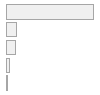
\includegraphics{./tmp/ds0013.png} & \vtop{\hbox{\strut 3407}\hbox{\strut (76.6\%)}} \\
Justificacion de violencia: Carabineros
desaloje liceos en toma (2019) & \vtop{\hbox{\strut Mean (sd) : 1.7 (1.1)}\hbox{\strut min \textless{} med \textless{} max:}\hbox{\strut 1 \textless{} 1 \textless{} 5}\hbox{\strut IQR (CV) : 1 (0.6)}} & \vtop{\hbox{\strut 1 : 2145 (63.3\%)}\hbox{\strut 2 : 549 (16.2\%)}\hbox{\strut 3 : 424 (12.5\%)}\hbox{\strut 4 : 161 ( 4.7\%)}\hbox{\strut 5 : 112 ( 3.3\%)}} & 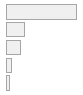
\includegraphics{./tmp/ds0014.png} & \vtop{\hbox{\strut 3391}\hbox{\strut (76.3\%)}} \\
Justificacion de violencia: Estudiantes
tiren piedras (2019) & \vtop{\hbox{\strut Mean (sd) : 1.5 (1)}\hbox{\strut min \textless{} med \textless{} max:}\hbox{\strut 1 \textless{} 1 \textless{} 5}\hbox{\strut IQR (CV) : 0 (0.6)}} & \vtop{\hbox{\strut 1 : 2554 (75.0\%)}\hbox{\strut 2 : 361 (10.6\%)}\hbox{\strut 3 : 285 ( 8.4\%)}\hbox{\strut 4 : 129 ( 3.8\%)}\hbox{\strut 5 : 76 ( 2.2\%)}} & 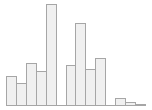
\includegraphics{./tmp/ds0015.png} & \vtop{\hbox{\strut 3405}\hbox{\strut (76.6\%)}} \\
Justificacion de violencia: Personas
dannien inmobiliario publico (2019) & \vtop{\hbox{\strut Mean (sd) : 1.3 (0.8)}\hbox{\strut min \textless{} med \textless{} max:}\hbox{\strut 1 \textless{} 1 \textless{} 5}\hbox{\strut IQR (CV) : 0 (0.6)}} & \vtop{\hbox{\strut 1 : 2849 (83.6\%)}\hbox{\strut 2 : 231 ( 6.8\%)}\hbox{\strut 3 : 212 ( 6.2\%)}\hbox{\strut 4 : 66 ( 1.9\%)}\hbox{\strut 5 : 48 ( 1.4\%)}} & 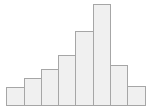
\includegraphics{./tmp/ds0016.png} & \vtop{\hbox{\strut 3406}\hbox{\strut (76.6\%)}} \\
Justificacion de violencia: Personas
dannien transporte (2019) & \vtop{\hbox{\strut Mean (sd) : 1.3 (0.7)}\hbox{\strut min \textless{} med \textless{} max:}\hbox{\strut 1 \textless{} 1 \textless{} 5}\hbox{\strut IQR (CV) : 0 (0.6)}} & \vtop{\hbox{\strut 1 : 2924 (85.8\%)}\hbox{\strut 2 : 214 ( 6.3\%)}\hbox{\strut 3 : 183 ( 5.4\%)}\hbox{\strut 4 : 45 ( 1.3\%)}\hbox{\strut 5 : 40 ( 1.2\%)}} & 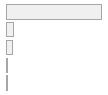
\includegraphics{./tmp/ds0017.png} & \vtop{\hbox{\strut 3406}\hbox{\strut (76.6\%)}} \\
Justificacion de violencia: Personas
dannien comercio (2019) & \vtop{\hbox{\strut Mean (sd) : 1.2 (0.6)}\hbox{\strut min \textless{} med \textless{} max:}\hbox{\strut 1 \textless{} 1 \textless{} 5}\hbox{\strut IQR (CV) : 0 (0.5)}} & \vtop{\hbox{\strut 1 : 3041 (89.4\%)}\hbox{\strut 2 : 178 ( 5.2\%)}\hbox{\strut 3 : 132 ( 3.9\%)}\hbox{\strut 4 : 24 ( 0.7\%)}\hbox{\strut 5 : 28 ( 0.8\%)}} & 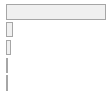
\includegraphics{./tmp/ds0018.png} & \vtop{\hbox{\strut 3403}\hbox{\strut (76.5\%)}} \\
\bottomrule
\end{longtable}

Existe una tendencia generalizada en los datos descriptivos univariados: más de la mitad de los encuestados considera que nunca se justifica la violencia, independiente de la situación, de los actores involucrados y del fin asociado. Sin embargo, al entrar en detalle se observa cómo los porcentajes varían de acuerdo con la situación. La situación que encuentra mayor justificación es que carabineros desalojen liceos en toma, con un 37.7\% asociado a algún grado de justificación. Los casos de represión a marchas pacíficas por parte de carabineros y lanzamiento de piedras desde estudiantes a carabineros presentan porcentajes parecidos, mientras un 21.8\% de encuestados señala que se justifica el actuar de carabineros, un 25\% de encuestados asevera que la táctica de los estudiantes está justificada. Esto muestra una muy leve tendencia a justificar más el actuar de los estudiantes, aunque sigue estando 10 puntos porcentuales abajo del desalojo a tomas por parte de carabineros. Las situaciones que muestren una tendencia mucho más consistente son las del daño a la propiedad. No más del 20\% de los encuestados justifica el daño a la propiedad, especialmente el daño a locales comerciales que presenta los niveles de justificación más bajos. Estos datos demarcan un panorama interesante para la profundización del análisis. Parece ser que si se comparan las dos tácticas más comunes en una situación de protesta (tanto de control como de protesta) no hay grandes variaciones en la justificación, sin embargo, cuando se consideran situaciones más excepcionales, la justificación por el control social aumenta, y por el cambio social disminuye. A modo de énfasis, llama la atención que pese al clima sostenido de protesta violenta durante los meses del estallido social \citep{Joignant2020}, la destrucción a la propiedad tenga tan baja justificación. Una posible explicación es que la propiedad es vista como un bien de uso público, por lo que su destrucción es perjudicial para la ciudadanía.

\begin{figure}[!ht]

{\centering 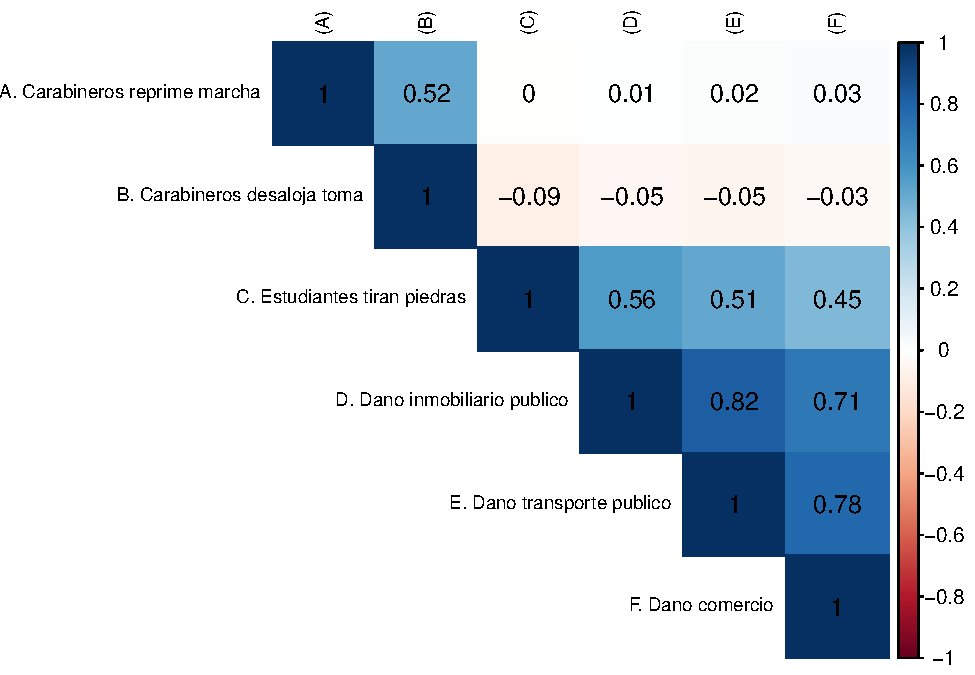
\includegraphics[width=1\linewidth,]{tesis_files/figure-latex/matpearson-1} 

}

\caption{Matriz de Correlaciones de Pearson  para Justificación Violencia}\label{fig:matpearson}
\end{figure}

\begin{figure}[!ht]

{\centering 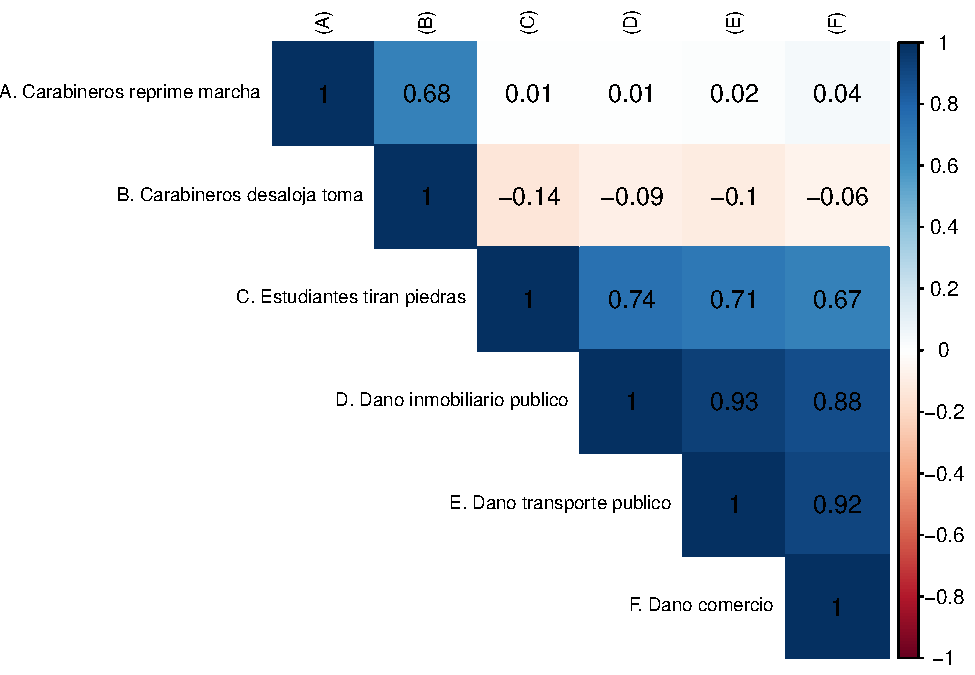
\includegraphics[width=1\linewidth,]{tesis_files/figure-latex/matpolycor-1} 

}

\caption{Matriz de Correlaciones Policlorica para Justificación Violencia}\label{fig:matpolycor}
\end{figure}

Las Figuras N° \ref{fig:matpearson} y N° \ref{fig:matpolycor} muestran las correlaciones de Pearson y policlóricas -respectivamente- para los indicadores de la variable dependiente. En general, la correlación entre indicadores es consistente con respecto a lo que se habría de esperar por la literatura. Los indicadores de carabineros, representando el concepto de violencia por el control social, correlacionan de forma positiva y moderada aproximándose a alta. Esto sustenta la idea de que aluden a un mismo concepto. En el caso de la violencia por el cambio social, el indicador de lanzamiento de piedras por parte de estudiantes es el que menos correlaciona con los otros del mismo concepto, aunque sigue siendo una correlación positiva moderada aproximándose a alta. Por el lado de los indicadores sobre la destrucción de la propiedad, estos correlacionan de forma positiva y bastante alta en ambas matrices de correlación, demostrando una vez más lo consistentes que son las respuestas con este tipo particular de violencia. Las correlaciones mayores a 0.9 en la Figura N° \ref{fig:matpolycor} llaman a la cautela y tener en cuenta qué tan distinto son los indicadores entre si, o si más bien los encuestados pensaban en las situaciones presentadas en cada indicador como parte de un todo. Esto llevaría a pensar en un factor latente por sí solo, o el uso de índices sumativos.

Estas matrices también aportan a evaluar las condiciones para un análisis factorial exploratorio (AFE). En general, las condiciones se cumplen en las matrices de Pearson y no en las policlóricas. En las primeras no hay correlaciones entre indicadores de un factor menores a 0.3 y mayores a 0.8, en cambio en las segundas sí. Se procede al análisis de más condiciones para determinar la aplicabilidad de un AFE.

\hypertarget{anuxe1lisis-factorial}{%
\section{Análisis factorial}\label{anuxe1lisis-factorial}}

Para analizar si están las condiciones para aplicar un AFE se efectúan tres pruebas: de normalidad, del determinante y el KMO. Para probar la hipótesis de normalidad se aplican dos pruebas: la de Kolmogorov-Smirnov con corrección de Lilliefors, dado que no se conoce ni la media ni la desviación estándar poblacional y se cuenta con una muestra mayor a 50 observaciones; y la de Jarque Bera a modo de complemento. Ambos test presentan valores \emph{p \textgreater{} 0.01}, por lo que se descarta el supuesto de normalidad. Por otro lado, el cálculo del determinante arroja un valor de 0.05797724, que siendo mayor al valor necesario de 0.00001 se cumple la condición para AFE. En esta línea, el KMO arroja un valor promedio de 0.75 para todos los indicadores, indicando que se cumplen las condiciones para un AFE.

Dado que se cumplen las condiciones, se procede a efectuar un AFE, sin embargo, como los datos no se distribuyen de forma normal se descarta la aplicación del método de estimación de Máxima Verosimilitud. En cambio, se opta por estimar los modelos a partir del Componente Principal y con rotación oblicua, lo que permite la correlación entre factores. El procedimiento es el siguiente: se estima un gráfico de sedimentación para analizar la cantidad de factores a usar según los \emph{eigenvalores}; independiente de lo anterior, se estiman cuatro modelos a modo exploratorio: uno de un factor, otro de dos factores, un tercer modelo de tres factores y un cuarto modelo con tres factores incluyendo un indicador que, hasta ahora, ha sido descartado por razones teóricas. Se finaliza analizando los indicadores de ajuste de los modelos.

\begin{figure}[!ht]

{\centering 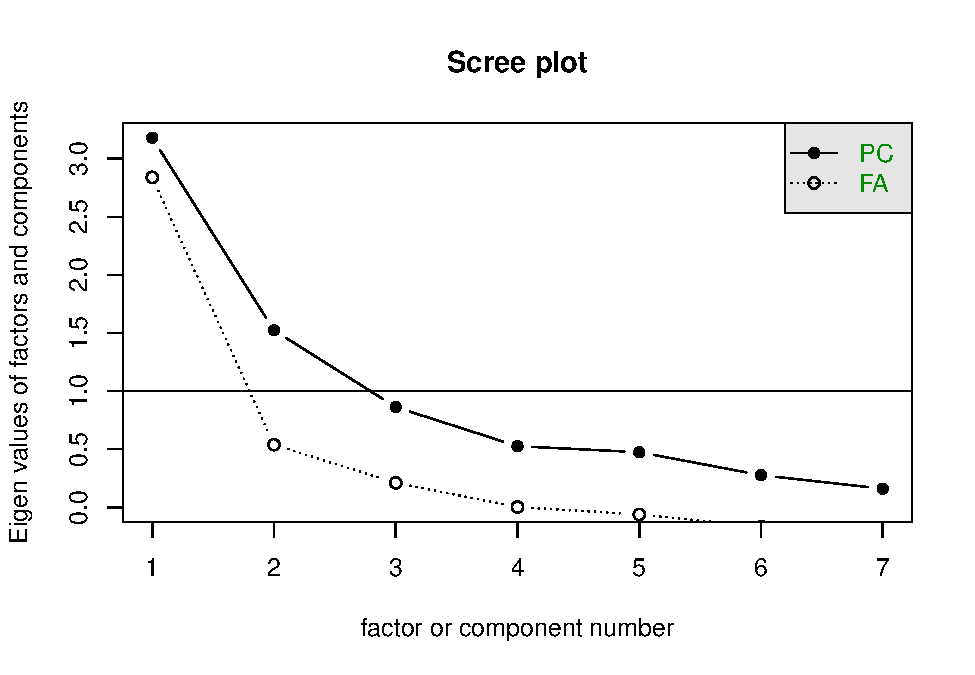
\includegraphics[width=1\linewidth,]{tesis_files/figure-latex/scree-1} 

}

\caption{Gráfico de Sedimentación para Análisis Factorial Exploratorio}\label{fig:scree}
\end{figure}

El gráfico de sedimentación presentado en la Figura N° \ref{fig:scree} muestra la cantidad de factores sugeridos según los eigenvalores. Los eigenvalores corresponden a una medida de cuánta varianza de las variables observada es explicada por un factor, siendo eigenvalores ≥ 1 cuando un factor logra explicar más que un indicador por si solo (regla de Kaiser). En este caso, el gráfico de sedimentación sugiere el uso de un factor con AFE, por lo que se comienza estimando un modelo de un factor. El modelo de un factor representado en la Tabla N° \ref{tab:f1t} muestra una distribución de cargas factoriales según lo que se habría esperar de la literatura: un factor no logra captar la violencia ejercida como táctica de protesta y aquella como forma de control. Las cargas de los indicadores de carabineros son básicamente 0, así como su unicidad es 1 o casi 1. Esta situación lleva a explorar modelos con más factores.

Las tablas N° \ref{tab:f2t} y N° \ref{tab:f3t} corresponden a los modelos de dos y tres factores respectivamente. El modelo de dos factores muestra una distribución de cargas factoriales consistente con la distinción de violencia por el cambio y violencia por el control social. Los indicadores de carabineros presentan cargas mayores a 0.7, en tanto los indicadores de destrucción a la propiedad presentan cargas arriba de 0.8 y el de estudiantes una carga de 0.5, todos con cargas cruzadas considerablemente pequeñas. Si bien todas las cargas son mayores a 0.3, por lo que se puede sostener la existencia de dos factores, llama la atención la gran diferencia entre la carga del indicador de estudiantes y los indicadores de propiedad, llevando a indagar en el modelo de tres factores. El modelo de tres factores también presenta una distribución de cargas lógica de acuerdo con una subdivisión del concepto de violencia por el cambio social. Con baja cargas cruzadas, el modelo muestra que la destrucción a la propiedad podría ser un factor por si mismo, en tanto el lanzamiento de piedras correspondería a otra dimensión del uso de la violencia. No obstante, se torna problemático un modelo de tres factores, donde un factor es solamente un indicador. Esto se evidencia en la Tabla N° \ref{tab:indf}, donde los indicadores de ajuste para este modelo no pudieron ser calculados. A modo de indagar más en la posibilidad de tres factores es que se introduce un indicador hasta ahora excluido por razones teóricas: la situación en la que trabajadores hacen barricadas para protestar por sus derechos.

Hasta ahora, considerando el rol que juega la concepción de la violencia en la justificación de esta \citep{Blumenthal1972} y a falta de una base empírica de qué es lo que los chilenos entienden por violencia, es que se optó por entender la violencia bajo un enfoque minimalista. El enfoque minimalista entiende la violencia como el uso intencional de la fuerza física que genera daño en quien lo recibe, a lo que dado el contexto de protesta y la clasificación de tácticas en la literatura de movimientos sociales se le agregó la destrucción de la propiedad \citep{Medel2016}. A raíz de esto, es que uno de los indicadores de la batería original de preguntas fue extraído, el cuál preguntaba por el grado de justificación para una situación en la que trabajadores hacían barricadas para luchar por sus derechos. Según la clasificación de tácticas de protesta, el armar barricadas o el hacer tomas cabe más dentro de la idea de tácticas disruptivas \citep{Medel2016}. No obstante, ante la posibilidad de un modelo de 3 factores, es que se agrega este indicador al análisis.

El modelo de tres factores más el indicador de trabajadores (Tabla N° \ref{tab:f3tt}) es consistente con el planteamiento de que la violencia por el cambio social se puede dividir en algo más de tipo disruptivo y la destrucción de la propiedad. Todas las cargas puntúan arriba de 0.7 y presentan cargas cruzadas bajas. El argumento de tres factores incluyendo este indicador se sostiene al ver los indicadores de ajuste en la Tabla N° \ref{tab:indf}, siendo este modelo el único que cumple todos los puntos limites que propone la literatura para los ajustes de AFE. Estos hallazgos abren la discusión sobre la conveniencia de utilizar puntajes factoriales para tres factores, o si mantener la conceptualización de dos tipos de violencia y estudiar los indicadores por separado para respetar las diferencias entre los indicadores de propiedad y de estudiantes. También llama a considerar el planteamiento teórico de la definición de violencia y su compatibilidad con la situación de barricadas. Previo a la toma de alguna decisión, un análisis factorial confirmatorio se hace esencial, así como también el tratamiento de los datos (dicotomización) para reducir el posible impacto de la poca varianza en los análisis.

\begin{table}

\caption{\label{tab:f1t}Cargas factoriales Modelo 1 Factor}
\centering
\begin{tabular}[t]{l|l|r|r|r}
\hline
  & JV & Communality & Uniqueness & Complexity\\
\hline
Dano Transporte. & 0.929 & 0.863 & 0.137 & 1\\
\hline
Dano Inmobiliario. & 0.9 & 0.810 & 0.190 & 1\\
\hline
Dano Locales & 0.809 & 0.655 & 0.345 & 1\\
\hline
Est. Piedras. & 0.581 & 0.338 & 0.662 & 1\\
\hline
Carab. Desalojo & -0.065 & 0.004 & 0.996 & 1\\
\hline
Carab. Represión & 0.001 & 0.000 & 1.000 & 1\\
\hline
\end{tabular}
\end{table}

\begin{table}

\caption{\label{tab:f2t}Cargas factoriales Modelo 2 Factores}
\centering
\begin{tabular}[t]{l|l|l|r|r|r}
\hline
  & JV. Cambio. & JV. Control & Communality & Uniqueness & Complexity\\
\hline
Dano Transporte. & 0.93 & 0.002 & 0.864 & 0.136 & 1.000\\
\hline
Dano Inmobiliario. & 0.9 & -0.006 & 0.810 & 0.190 & 1.000\\
\hline
Dano Locales & 0.81 & 0.024 & 0.656 & 0.344 & 1.002\\
\hline
Est. Piedras. & 0.578 & -0.051 & 0.339 & 0.661 & 1.015\\
\hline
Carab. Desalojo & -0.038 & 0.73 & 0.536 & 0.464 & 1.005\\
\hline
Carab. Represión & 0.041 & 0.712 & 0.506 & 0.494 & 1.007\\
\hline
\end{tabular}
\end{table}

\begin{table}

\caption{\label{tab:f3t}Cargas factoriales Modelo 3 Factores}
\centering
\begin{tabular}[t]{l|l|l|l|r|r|r}
\hline
  & JV. Destruccion prop. & JV Control & JV. Protesta disruptiva & Communality & Uniqueness & Complexity\\
\hline
Dano Transporte. & 0.988 & -0.011 & -0.045 & 0.913 & 0.087 & 1.004\\
\hline
Dano Locales & 0.83 & 0.015 & -0.014 & 0.672 & 0.328 & 1.001\\
\hline
Dano Inmobiliario. & 0.66 & 0.005 & 0.283 & 0.794 & 0.206 & 1.356\\
\hline
Carab. Desalojo & 0.014 & 0.729 & -0.064 & 0.541 & 0.459 & 1.016\\
\hline
Carab. Represión & -0.014 & 0.715 & 0.064 & 0.508 & 0.492 & 1.017\\
\hline
Est. Piedras. & 0.064 & -0.015 & 0.656 & 0.499 & 0.501 & 1.020\\
\hline
\end{tabular}
\end{table}

\begin{table}

\caption{\label{tab:f3tt}Cargas factoriales Modelo 3 Factores + Indicador Trabajo}
\centering
\begin{tabular}[t]{l|l|l|l|r|r|r}
\hline
  & JV. Destruccion prop. & JV. Control & JV. Protesta disruptiva & Communality & Uniqueness & Complexity\\
\hline
Dano Transporte. & 0.976 & -0.012 & -0.039 & 0.903 & 0.097 & 1.003\\
\hline
Dano Locales & 0.848 & 0.012 & -0.038 & 0.677 & 0.323 & 1.004\\
\hline
Dano Inmobiliario. & 0.741 & 0.005 & 0.193 & 0.781 & 0.219 & 1.136\\
\hline
Carab. Represión & -0.003 & 0.723 & 0.051 & 0.519 & 0.481 & 1.010\\
\hline
Carab. Desalojo & 0.001 & 0.72 & -0.054 & 0.529 & 0.471 & 1.011\\
\hline
Est. Piedras. & 0.091 & 0.004 & 0.689 & 0.568 & 0.432 & 1.035\\
\hline
Trab. Barricada & -0.058 & -0.021 & 0.617 & 0.339 & 0.661 & 1.020\\
\hline
\end{tabular}
\end{table}

\begin{table}

\caption{\label{tab:indf}Ajuste Modelos Análisis Factorial Exploratorio}
\centering
\begin{tabular}[t]{l|r|r|r|r}
\hline
Indicador Ajuste & Modelo 1F & Modelo 2F & Modelo 3F & Modelo 3 F + Indicador Trabajadores\\
\hline
TLI & 0.787 & 0.938 & NA & 0.997\\
\hline
RMSEA & 0.201 & 0.108 & NA & 0.022\\
\hline
RMSR & 0.140 & 0.020 & 0 & 0.000\\
\hline
RMSR & 1556.840 & 179.120 & NA & -15.600\\
\hline
\end{tabular}
\end{table}

\hypertarget{anuxe1lisis-multivariado}{%
\section{Análisis multivariado}\label{anuxe1lisis-multivariado}}

\hypertarget{conclusiones}{%
\chapter{Conclusiones}\label{conclusiones}}

\hypertarget{bibliografuxeda}{%
\chapter*{Bibliografía}\label{bibliografuxeda}}
\addcontentsline{toc}{chapter}{Bibliografía}

% %%%%%%%%%%%%%%%%%%%%%%%%%%%%%%%%%%%%%%%%%%%%%%%%%
% %%% Bibliography                              %%%
% %%%%%%%%%%%%%%%%%%%%%%%%%%%%%%%%%%%%%%%%%%%%%%%%%
% \addtocontents{toc}{\vspace{.5\baselineskip}}
% \cleardoublepage
% \phantomsection
% \addcontentsline{toc}{chapter}{\protect\numberline{}{Bibliography}}
\bibliography{tesis}

%% All books from our library (SfS) are already in a BiBTeX file
%% (Assbib). You can use Assbib combined with your personal BiBTeX file:
%% \bibliography{Myreferences,Assbib}. Of course, this will only work on
%% the computers at SfS, unless you copy the Assbib file
%%  --> /u/sfs/bib/Assbib.bib



\end{document}
